\documentclass{article}

% 33.1 inches by 46.8 inches
% 841 mm by 1189 mm
\usepackage[a0paper, landscape,  margin=.5in]{geometry}
\usepackage{amsmath}
\usepackage{tikz}

\setlength{\parindent}{0pt}

\begin{document}

\begin{center}
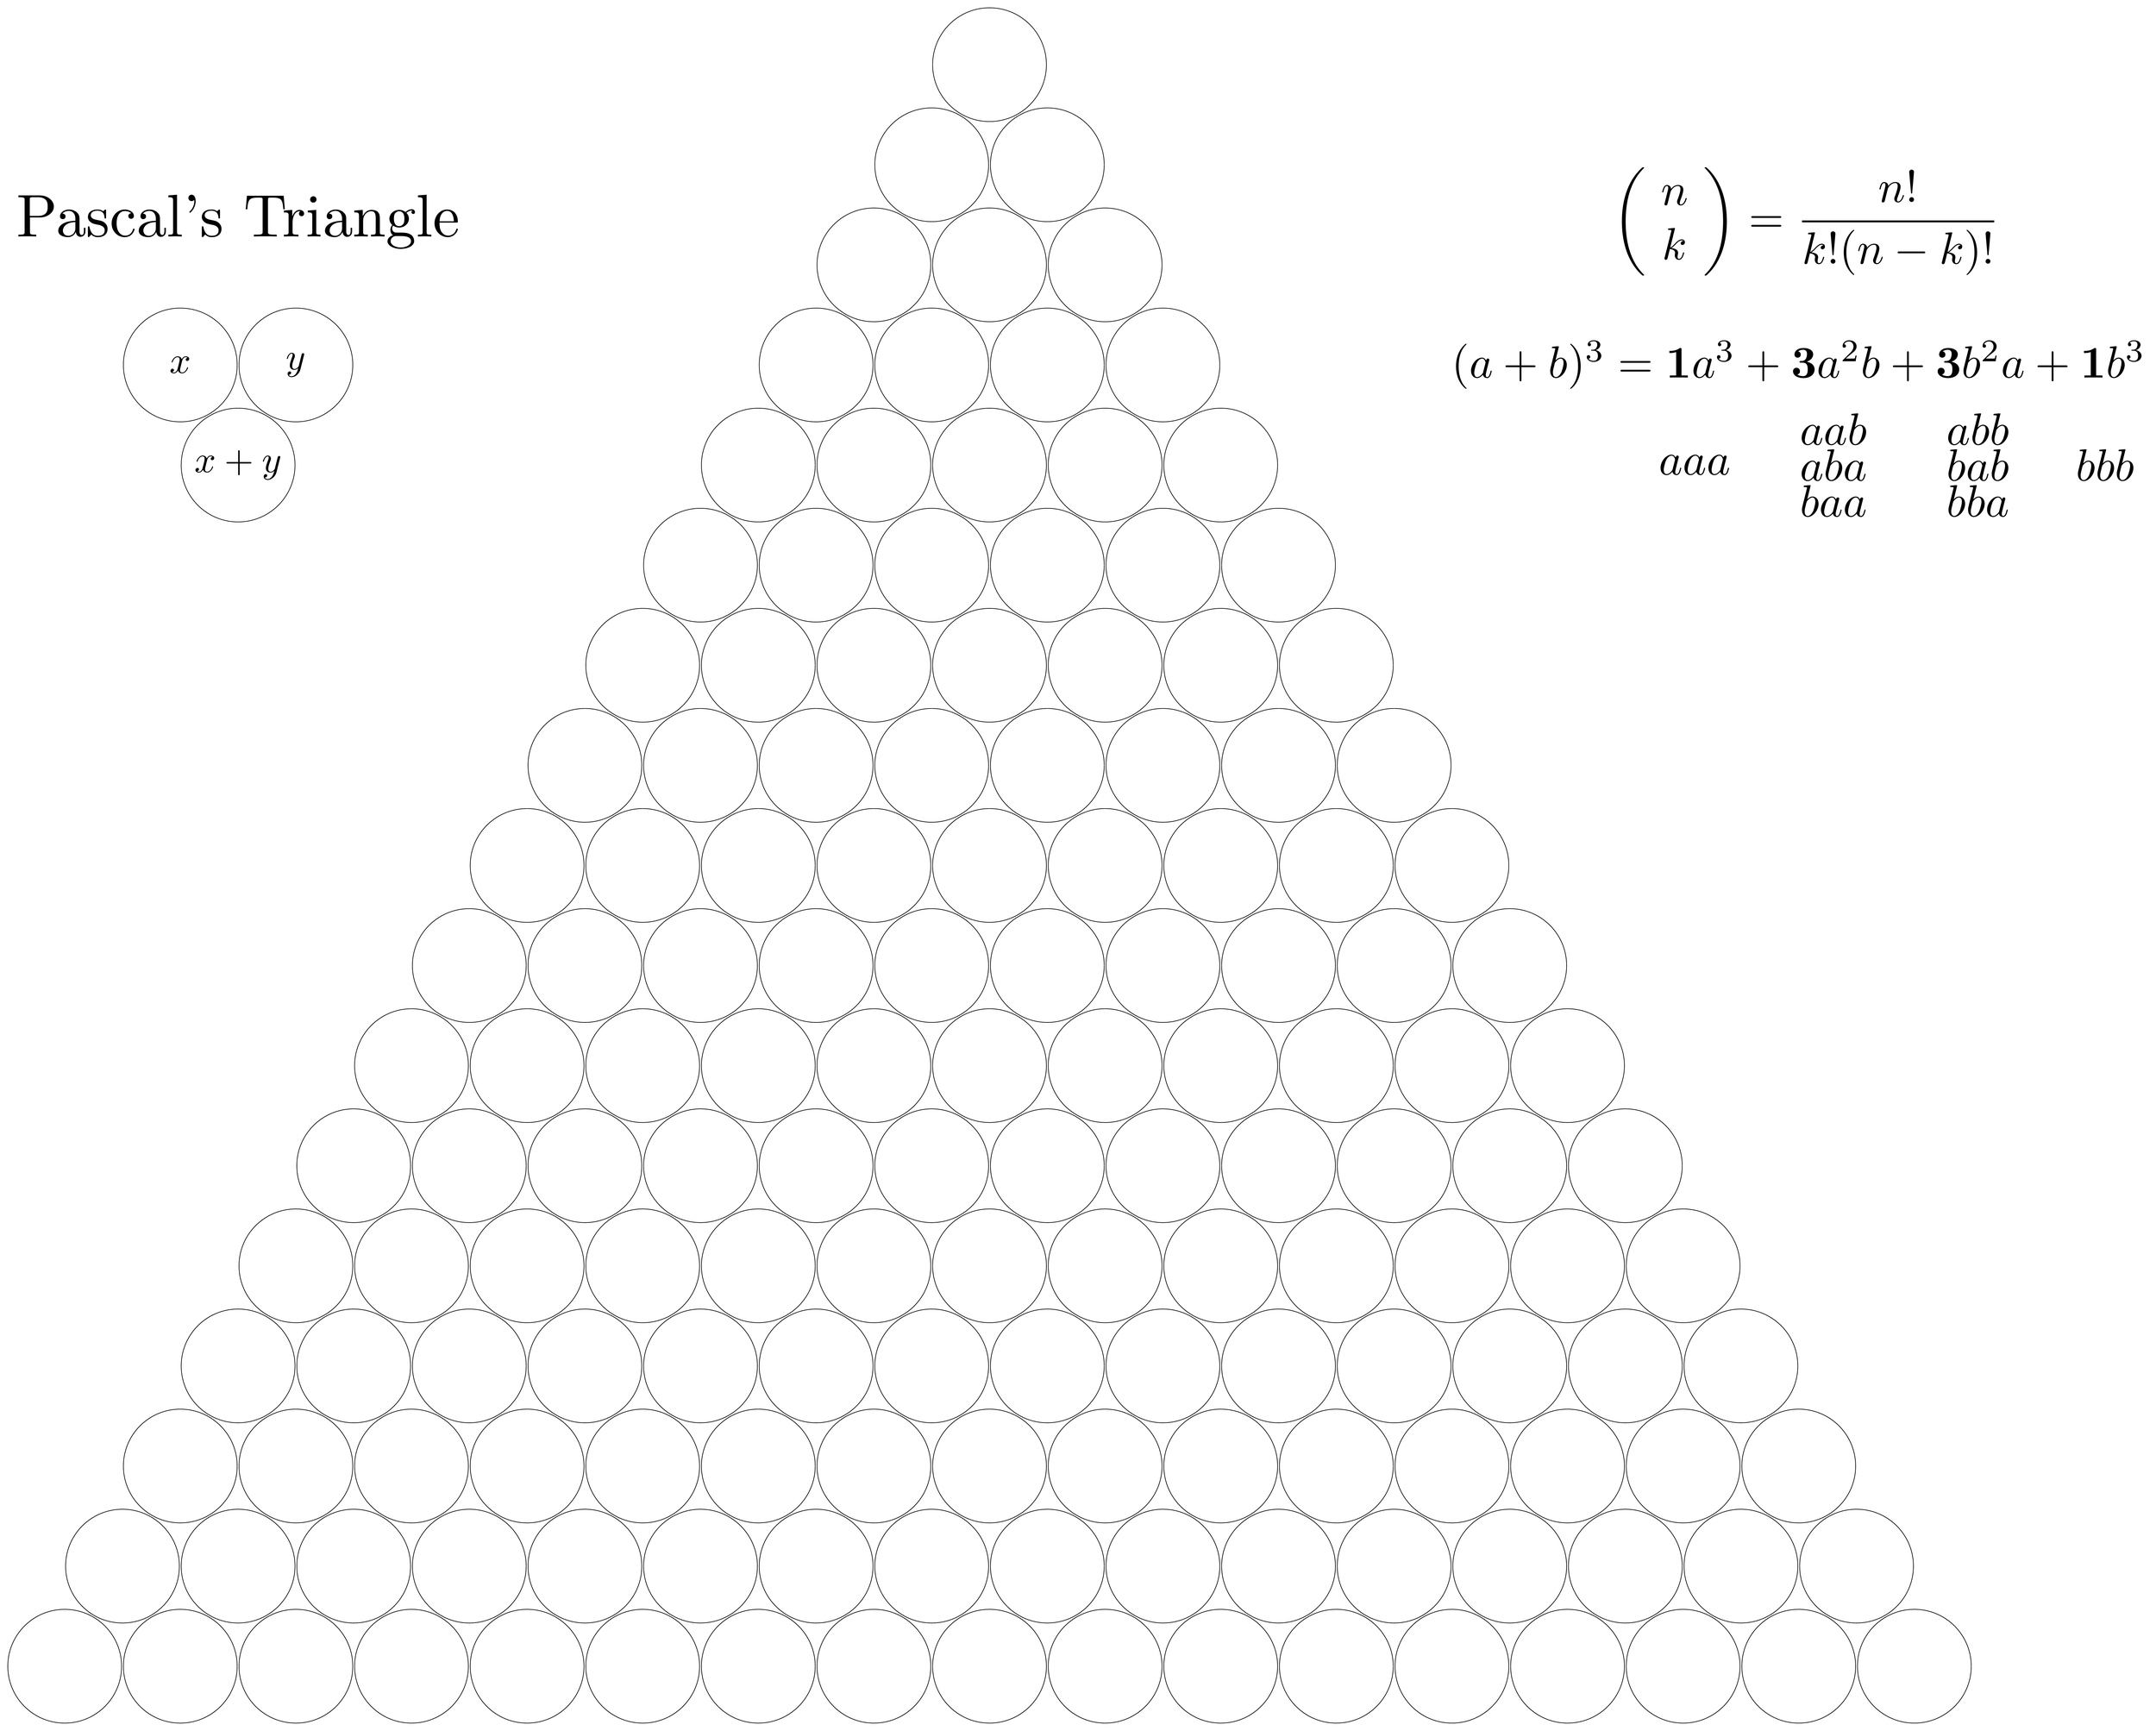
\begin{tikzpicture}[scale=5.4]
  \def\radius{14pt}
  \node (title) at (-6.5, 12.5) {\scalebox{8}{Pascal's Triangle}};
  \draw[thick] (-7, 13 *.866025) circle (\radius);
  \draw[thick] (-6, 13 *.866025) circle (\radius);
  \draw[thick] (-6.5, 12 *.866025) circle (\radius);

  \node (equation) at (7, 12.5) {\scalebox{6}{
    $\left(\! \begin{array}{c} n\\k \end{array} \!\right) = \displaystyle\frac{n!}{k! (n-k)!}$}};

\node (equation1) at (7, 13 * .866025) {\scalebox{6}{%
    $(a + b)^3 = \mathbf{1} a^3 + \mathbf{3} a^2 b + \mathbf{3} b^2 a + \mathbf{1} b^3$}};

\node (equation3) at (6.1, 12 * .866025) {\scalebox{6}{$aaa$}};
\node (equation3) at (7.3, 12 * .866025) {\scalebox{6}{$\substack{\displaystyle aab\\\displaystyle aba\\\displaystyle baa}$}};
\node (equation3) at (8.55, 12 * .866025) {\scalebox{6}{$\substack{\displaystyle abb\\\displaystyle bab\\\displaystyle bba}$}};
\node (equation3) at (9.65, 12 * .866025) {\scalebox{6}{$bbb$}};

  \node (a) at (-7, 13 * .866025) {\scalebox{5}{$x$}};
  \node (a) at (-6, 13 * .866025) {\scalebox{5}{$y$}};
  \node (a) at (-6.5, 12 * .866025) {\scalebox{5}{$x+y$}};
  \foreach \i in {0,...,16} {
    \foreach \j in {0,...,\i} {
      % 16 * sqrt(3) / 2 = 13.8564
      \draw[thick] (\j - .5 * \i, 13.8564 - \i * .866025) circle (\radius);
    }
  }
\end{tikzpicture}
\end{center}

\end{document}
